\chapter{Data science project}
\label{chap:project}

% TODO: do not forget to talk about documentation and deployment

\chapterprecishere{\raggedleft\textup{with contributions from} \textsc{Johnny C. Marques}
  \\[5mm] Figured I could throw myself a pity party or go back to school and learn the computers.
  \par\raggedleft--- \textup{Don Carlton}, Monsters University (2013)}

First of all, \emph{a data science project is a software project}.  The difference between a data
science software and a traditional software is that some components of the former are
constructed from data.  This means that part of the solution is not designed from the
knowledge of the domain expert.

One example of project is a spam filter that
classifies emails into two categories: spam and non-spam.  A traditional approach is
to design a set of rules that are known to be effective.  However, the effectiveness of
the filters is limited by the knowledge of the designer and is cumbersome to maintain.  A
data science approach automatically learns the filters from a set of
emails that are already classified as spam or non-spam.

Another important difference in data science projects is that traditional testing methods,
such as unit tests, are not enough.  The solution inferred from the data must be validated
considering the stochastic nature of the data.

In this chapter, we discuss common methodologies for data science projects.  We also
present the concept of agile methodologies and the Scrum framework.  We finally propose an
extension to Scrum adapted for data science projects.

\begin{mainbox}{Chapter remarks}

  \boxsubtitle{Contents}

  \startcontents[chapters]
  \printcontents[chapters]{}{1}{}
  \vspace{1em}

  \boxsubtitle{Context}

  \begin{itemize}
    \itemsep0em
    \item Data science project is a software project.
    \item Data science methodologies focus on the data analysis process.
    \item Industry demands not only data analysis but also software development.
  \end{itemize}

  \boxsubtitle{Objectives}

  \begin{itemize}
    \itemsep0em
    \item Explore the common methodologies for data science projects.
    \item Understand the agile methodologies and the Scrum framework.
    \item Propose an extension to Scrum adapted for data science projects.
  \end{itemize}

  \boxsubtitle{Takeways}

  \begin{itemize}
    \itemsep0em
    \item Good methodologies take into account the software development aspects of the
      project.
    \item Scrum is a good framework for software development, and it can be adapted for
      data science projects.
  \end{itemize}
\end{mainbox}

{}
\clearpage

\section{CRISP-DM}

CRISP-DM\footnote{Official guide available at
\url{https://www.ibm.com/docs/it/SS3RA7_18.3.0/pdf/ModelerCRISPDM.pdf}.} is a methodology
for data mining projects.  It is an acronym for Cross Industry Standard Process for Data
Mining.  It is a methodology that was developed in the 1990s by IBM, and it is still
widely used today.

CRISP-DM is a cyclic process.  The process is composed of six phases:
\begin{enumerate}
  \item Business understanding: this is the phase where the project objectives are
    defined.  The objectives must be defined in a way that is measurable.  The phase also
    includes the definition of the project plan.
  \item Data understanding: this is the phase where the data is collected and explored.
    The data is collected from the data sources, and it is explored to understand its
    characteristics.  The phase also includes the definition of the data quality
    requirements.
  \item Data preparation: this is the phase where the data is prepared for the modeling
    phase.  The data is cleaned, transformed, and aggregated.  The phase also includes the
    definition of the modeling requirements.
  \item Modeling: this is the phase where the model is trained and validated.  The model is
    trained using the prepared data, and it is validated using the validation data.  The
    phase also includes the definition of the evaluation requirements.
  \item Evaluation: this is the phase where the model is evaluated.  The model is evaluated
    using the evaluation data.  The phase also includes the definition of the deployment
    requirements.
  \item Deployment: this is the phase where the model is deployed.  The model is deployed
    using the deployment requirements.  The phase also includes the definition of the
    monitoring requirements.
\end{enumerate}

CRISP-DM is cyclic and completly focused on the data.  However, it does not address the
software development aspects of the project.  The ``product'' of the project is both
models and findings, not the full software solution.  As a result, aspects such as user
interface, communication and integration are not addressed by the methodology.

\clearpage

\begin{figurebox}[label=fig:cripdm]{Diagram of the CRISP-DM process.}
  \centering
  \begin{tikzpicture}
    \node (1) at (0, 0) {};
    \node (2) at (4, -4) {};
    \node (3) at (0, -8) {};
    \node (4) at (-4, -4) {};

    \node [block] (bu) at (-1.5, -2) {Business understanding};
    \node [block] (du) at (1.5, -2) {Data understanding};
    \path [line] (bu) -- (du);
    \path [line] (du) -- (bu);

    \node [block] (dp) at (2.5, -3.5) {Data preparation};
    \node [block] (m) at (2.5, -5) {Modeling};
    \path [line] (dp) -- (m);
    \path [line] (m) -- (dp);

    \path [line] (du) -- (dp);

    \node [block] (e) at (0, -6.5) {Evaluation};
    \node [block] (d) at (-2.5, -4.25) {Deployment};

    \path [line] (m) -- (e);
    \path [line] (e) -- (d);
    \path [line] (e) -- (bu);

    \node [draw, circle, fill=gray, text centered, text=white] at (0, -4.25) {Data};

    \path [bigarrow] (1.east) to[out=0, in=90] (2.60);
    \path [bigarrow] (2.-60) to[out=-90, in=0] (3.east);
    \path [bigarrow] (3.west) to[out=180, in=-90] (4.-120);
    \path [bigarrow] (4.120) to[out=90, in=180] (1.west);
  \end{tikzpicture}
  \tcblower
  Each block represents a phase of the CRISP-DM process.  Data is the central element of
  the process.  Arrows represent the transitions between the phases.
\end{figurebox}

\Cref{fig:cripdm} shows a diagram of the CRISP-DM process.  The double arrow between the
business understanding and the data understanding phases represents the iterative nature
of these steps.  Once we are satisfied with the data understanding, we can go further to
the data preparation phase.  The same iteration is possible between the data preparation
and the modeling phases, since modeling methods can require different data preparation
methods. Finally, an evaluation is performed.  If the model is satisfactory, we go to the
deployment phase.  Otherwise, we go back to the business understanding phase.  The idea
to go back to the business understanding phase is to rethink the project objectives.% and
% the project plan.

The CRISP-DM methodology is a good starting point for data science projects.  However, it
does not mean that should be followed strictly.  The process is flexible, and
adaptations are possible at any stage.

\section{ZM approach}

\textcite{Zumel2019}\footfullcite{Zumel2019} also propose a methodology for data science projects --- which we
call the ZM approach.  Besides
describing each step in a data science project, they further address the roles of each
individual involved in the project.  They state that data science projects are always
collaborative, as they require domain expertise, data expertise, and software expertise.

Requirements of a data science project are dynamic, and we need to perform many
exploratory phases.  Unlike traditional software projects, we should expect the
great changes in the initial requirements and project goals.

Usually,
projects based on data are urgent, and they must be completed in a short time --- not
only due to the business requirements, but also because the data changes over time.
The authors state that agile methodologies are suitable (and necessary) for data science
projects.

\subsection{Roles of the ZM approach}

In their approach, they define five roles.  The roles are:

\paragraph{Project sponsor}  It is the main stakeholder of the project, the one that needs the
results of the project.  He represents the business interests and champions the project.
The project is considered successful if the sponsor is satisfied.  Note that, ideally, the
sponsor can not be the data scientist, but someone that is not involved in the development
of the project.  However, he needs to be able to express \emph{quantitatively} the business
goals and participate actively in the project.

\paragraph{Client}  The client is the domain expert.  He represents the end users'
interests.  In a small project, he is usually the sponsor.  He translates the daily
activities of the business into the technical requirements of the software.

\paragraph{Data scientist}  The data scientist is the one that sets and executes the
analytic strategy.  He is the one that communicates with the sponsor and the client,
effectively connecting all the roles.  In small projects, he can also act as the developer
of the software.  However, in large projects, he is usually the project manager.
Although it is not required to be a domain expert, the data scientist must be able to
understand the domain of the problem.  He must be able to understand the business goals and
the client's requirements.  Most importantly, he must be able to define and to solve the
right tasks.

\paragraph{Data architect}  The data architect is the one that manages data and data storage.
He usually is involved in more than one project, so it is not an active participant.  He
that receives instructions to adapt the data storage and means to collect data.

\paragraph{Operations}  The operations role is the one that manages infrastructure and
deploys final project results.  He is responsible to define requirements such as response
time, programming language, and the infrastructure to run the software.

\subsection{Processes of the ZM approach}

\citeauthor{Zumel2019}'s model is similar to CRISP-DM, but emphasizes that back-and-forth
is possible at any stage of the process.  \Cref{fig:zumel} shows a diagram of the process.
The phases and the answers we are looking for in each phase are:
\begin{itemize}
  \itemsep0em
  \item Define the goal: what problem are we trying to solve?
  \item Collect and manage data: what information do we need?
  \item Build the model: what patterns in the data that may solve the problem?
  \item Evaluate the model: is the model good enough to solve the problem?
  \item Present results and document: how did we solve the problem?
  \item Deploy the model: how to use the solution?
\end{itemize}

The step ``Present results and document'' is a differentiator from other approaches, like
CRISP-DM.  In ZM approach, result presentation is essential; data scientists must be able
to communicate their results effectively to the client/sponsor.  This phase is also
emphasized in the view of \textcite{Wickham2023}.

\begin{figurebox}[label=fig:zumel]{Diagram of the data science process proposed by \textcite{Zumel2019}.}
  \centering
  \begin{tikzpicture}
    \node (1) at (0, 0) {};
    \node (2) at (1, -1) {};
    \node (3) at (0, -2) {};
    \node (4) at (-1, -1) {};
    \path [bigarrow] (1.east) to[out=0, in=90] (2.60);
    \path [bigarrow] (2.-60) to[out=-90, in=0] (3.east);
    \path [bigarrow] (3.west) to[out=180, in=-90] (4.-120);
    \path [bigarrow] (4.120) to[out=90, in=180] (1.west);

    \node [block] (dg) at (0, 1) {Define the goal};
    \node [block] (cm) at (3, -0.25) {Collect and manage data};
    \node [block] (bm) at (3, -1.75) {Build the model};
    \node [block] (em) at (0, -3) {Evaluate the model};
    \node [block] (pd) at (-3, -1.75) {Present results};
    \node [block] (dm) at (-3, -0.25) {Deploy the model};

    \path [dline] (dg) to[out=0, in=90] (cm.north);
    \path [dline] (cm) -- (bm);
    \path [dline] (bm.south) to[out=-90, in=0] (em.east);
    \path [dline] (em.west) to[out=180, in=-90] (pd.south);
    \path [dline] (pd) -- (dm);
    \path [dline] (dm.north) to[in=180, out=90] (dg.west);
  \end{tikzpicture}

  \tcblower
  Each block represents a phase of the data science process.  The emphasis is on the
  cyclic nature of the process.  Arrows represent the transitions between the phases, that
  can be back-and-forth.
\end{figurebox}

\section{Agile methodology}

Agile is a methodology for software development.  It is an alternative to the waterfall
methodology.  The waterfall methodology is a sequential design where each phase
must be completed before the next phase can begin.

The methodology is based on the four values of agile manifesto\footnote{\url{https://agilemanifesto.org/}}:
\begin{itemize}
  \itemsep0em
  \item Individuals and interactions over processes and tools;
  \item Working software over comprehensive documentation;
  \item Customer collaboration over contract negotiation;
  \item Responding to change over following a plan.
\end{itemize}

Note that the manifesto does not discard the items on the right, but values the items on
the left more.  For example, comprehensive documentation is important, but working software
is more important.

\section{Scrum framework}

The Scrum framework is one of the most widely adopted agile methodologies. It is an
iterative, incremental process that enables teams to deliver high-value products
efficiently while adapting to changing requirements. Scrum emphasizes teamwork,
accountability, and continuous improvement. Developed by Ken Schwaber and Jeff Sutherland
in the early 1990s, Scrum is based on three pillars: transparency, inspection, and
adaptation. These principles help teams to navigate complex, adaptive problems and deliver
productive outcomes \parencite{schwaber2020scrum}.

Scrum organizes work into cycles called Sprints, and involves defined roles, ceremonies,
and artifacts that ensure the progress and quality of the product. Key events such as
daily stand-ups, sprint reviews, and retrospectives create regular opportunities to inspect
and adapt, making Scrum a responsive and resilient framework \parencite{denning2016scrum}.

\subsection{Scrum roles}

Scrum defines three critical roles: the Product Owner, the Scrum Master, and the
Development Team.

\begin{itemize}
  \item Product Owner: This role is responsible for defining the product vision and
    maximizing the value of the work done by the team. The Product Owner manages the
    Product Backlog, ensuring that it is visible, transparent, and prioritized according
    to business needs. They serve as the main point of contact between stakeholders and
    the development team \parencite{openagile2019roles}. The Product Owner must constantly
    balance the requirements of the business and the technical capabilities of the team,
    ensuring that the highest-value items are worked on first.
  \item Scrum Master: The Scrum Master acts as a facilitator and coach for the Scrum team,
    ensuring that the team adheres to the Scrum framework and agile principles. Unlike a
    traditional project manager, the Scrum Master is not responsible for managing the team
    directly but for enabling them to perform optimally by removing impediments and
    fostering a self-organizing culture \parencite{cobb2015scrum}.
  \item Development Team: The Development Team is a cross-functional group of professionals
    responsible for delivering potentially shippable product increments at the end of each
    sprint. The team is self-managing, meaning they decide how to achieve their goals
    within the sprint. The team should be small enough to remain nimble but large enough
    to complete meaningful work \parencite{rubin2012sprints}. The Development Team works
    collaboratively and takes collective responsibility for the outcome of the sprint.
\end{itemize}

Each of these roles has specific responsibilities, and together they ensure that the Scrum
process runs smoothly and that the product development aligns with the overall business
objectives.

\subsection{Sprints and backlog}

A Sprint is the basic unit of work in Scrum, as presented in \cref{fig:scrum}. Sprints
are time-boxed iterations, usually lasting between one to four weeks, during which a
defined amount of work is completed. The goal is to deliver a potentially shippable
product increment at the end of each sprint. Sprints are continuous, with no breaks in
between, fostering a regular, predictable rhythm of work \parencite{cobb2015scrum}.

% TODO: rewrite in TikZ
\begin{figure}
    \centering
    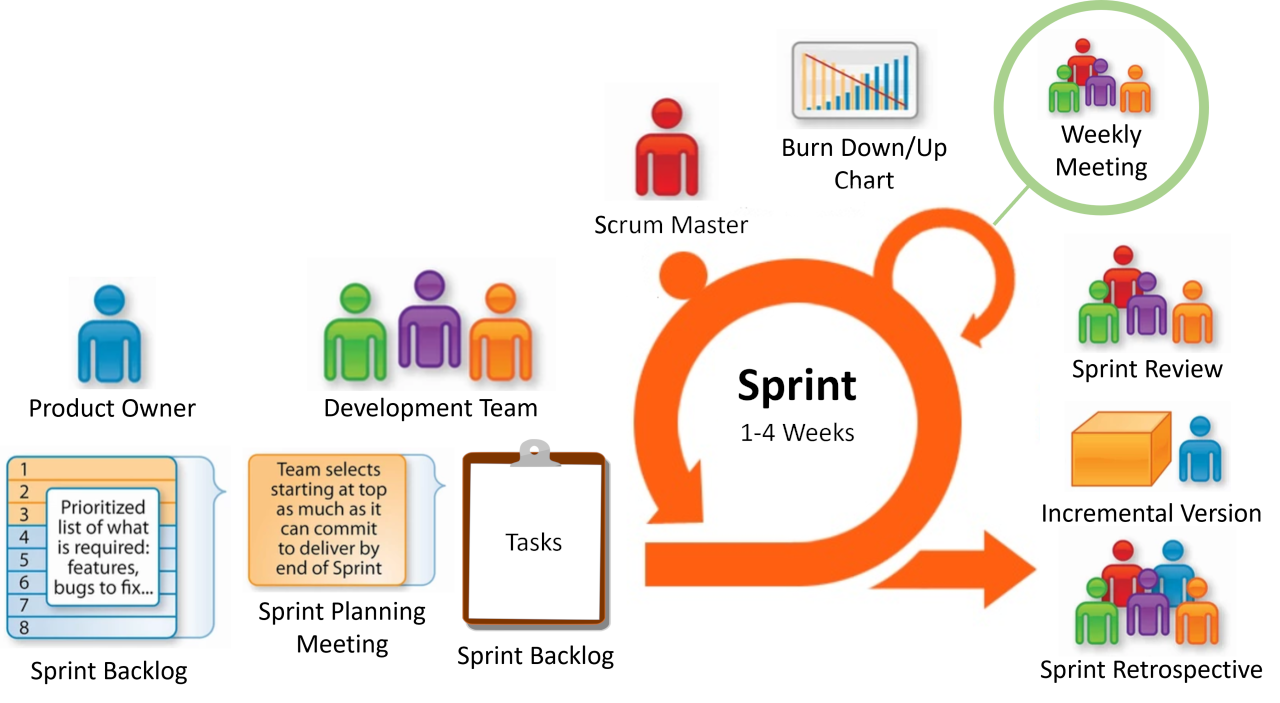
\includegraphics[width=1\linewidth]{images/scrum.png}
    \caption{Scrum Framework.}
    \label{fig:scrum}
\end{figure}

Before a sprint starts, the Scrum team holds a Sprint Planning meeting to decide what will
be worked on. The work for the sprint is selected from the Product Backlog, which is a
prioritized list of features, enhancements, bug fixes, and other deliverables necessary
for the product \parencite{schwaber2020scrum}. The Product Backlog is dynamic and evolves as
new requirements and changes emerge. The items selected for the sprint become part of the
Sprint Backlog, a subset of the Product Backlog that the Development Team commits to
completing during the sprint.

At the heart of the Scrum process is the Daily Scrum (or stand-up meeting), a brief
meeting where the team discusses progress toward the sprint goal, any obstacles they are
facing, and their plans for the next day. This daily inspection ensures that everyone
stays aligned and can quickly adapt to any changes or challenges \parencite{cobb2015scrum}.

The Burn Down/Up Chart is a visual tool widely used during the Sprint to track the Scrum
team's progress against the planned tasks. It displays the amount of remaining work (in
hours or story points) over time, allowing the team and the Product Owner to monitor
whether the work is on pace to be completed by the end of the sprint. The chart's line
decreases as tasks are finished, providing a clear indicator of potential delays or
blockers. If progress is falling behind, the team can adjust their approach during the
sprint by re-prioritizing tasks or removing impediments. Thus, the burn-down chart provides
real-time visibility into the team’s efficiency and contributes to more agile and
proactive work management.

At the end of each sprint, the team holds a Sprint Review, during which they demonstrate
the work completed during the sprint. The Sprint Review is an opportunity for stakeholders
to see progress and provide feedback, which may lead to adjustments in the Product
Backlog. Following the review, the team conducts a Sprint Retrospective to discuss what
went well, what didn't, and how they can improve their processes moving forward
\parencite{rubin2012sprints}. These continuous improvement cycles are key to Scrum's success,
allowing teams to adapt both their work and their working methods iteratively.

The Sprint Retrospective is a crucial event in the Scrum framework, held at the end of
each sprint. Its primary purpose is to provide the Scrum team with an opportunity to
reflect on the sprint that just concluded and identify areas for improvement. During the
retrospective, the team discusses what went well, what challenges they encountered, and
how they can enhance their processes for future sprints. This continuous improvement focus
allows the team to adapt their workflow and collaboration methods, fostering a more
efficient and effective development cycle. By encouraging open and honest feedback, the
retrospective plays a vital role in maintaining team cohesion and driving productivity
over time.

\subsection{Scrum for data science projects}

Some consider that Scrum is not adequate for data science projects.  The main reason is
that Scrum is designed for projects where the requirements are known in advance.  Also,
that data science projects have exploratory phases, which are not well supported by Scrum.

I argue that this view is wrong.  Scrum is a framework, and it is designed to be adapted to
the needs of the project;  Scrum is not a rigid process.  In the following, I propose an
extension to Scrum that makes it suitable for data science projects\footnote{Note that
many other adaptations to Scrum have been described in literature.  For example,
\fullcite{Saltz2019,Baijens2020,Kraut2022}.}.

One of my major concerns in the proposal of the extension is that data science projects
usually involve ``data scientists'' that are primarily developers, but statisticians or
domain-experts.  They usually do not ``hacking-level'' skills, and they often do not know
good practices of software development.

Scrum is a good starting point for a compromise between the need for autonomy (required in
dynamic and exploratory projects) and the need for a detailed plan to guide the project
(required to avoid bad practices and low quality software). A good project methodology is
needed to ensure that the project is completed in time and within budget.

\section{Our approach}

The previously mentioned methodologies lack the focus on the software development aspects of
the data science project.  For instance, CRISP-DM defines the stages only of the data
mining process, i.e. it does not explicitly address user interface or data collection.
\citeauthor{Zumel2019}'s approach addresses data collection and presentation of results, but
delegates the software development to the operations role, barely mentioning it.  Scrum is
a good framework for software development, but it is not designed for data science
projects.  For instance, it lacks the exploratory phases of data science projects.

Thus, we propose an extension to Scrum that makes it suitable for data science projects.
The extension is based on the following observations:
\begin{itemize}
  \itemsep0em
  \item Data science projects have exploratory phases;
  \item Data itself is a component of the solution;
  \item The solution is usually modularized, parts of it are constructed from data while the
    other parts are constructed like traditional software;
  \item The solution is usually deployed as a service, that must be maintained and
    monitored;
  \item Team members not familiar with software development practices must be guided to
    produce high-quality software.
\end{itemize}

Moreover, we add two other values besides the agile manifesto values.  They are:
\begin{itemize}
  \itemsep0em
  \item Confidence and understanding of the model over performance;
  \item Code version control over interactive environments.
\end{itemize}

The first value is based on the observation that the model performance is not the most
important aspect of the model.  The most important aspect is the being sure that the model
behaves as expected (and sometimes why it behaves as expected).  It is not uncommon to find
models that seems to perform well during evaluation steps\footnote{Of course, when
evaluation is not performed correctly.}, but that are not suitable for production.

The second value is based on the observation that interactive environments are not suitable
for the development of consistent and reproducible software solutions.  Interactive environments
help in the exploratory phases, but the final version of the code must be version
controlled.  Often, we hear stories that models cannot be reproduced because the code that
generated them are not runnable anymore.  This is a serious problem, and it is not
acceptable for maintaining a software solution.

As in the agile manifesto, the values on the right are not discarded, but the values on the
left are more important.  We do not discard the importance of model performance or the
convenience of interactive environments, but they are not the most important aspects of the
project.

These observations and values are the basis of our approach.  The roles and principles of
our approach are described in the following sections.

\subsection{The roles of our approach}

Although the roles of the ZM approach consider people potentially from different
organizations and the roles of Scrum focus on the development team, we can associate the
responsibilities between them.

Parts of the responsibilities of the product owner (that represents the stakeholders) in a
Scrum project are divided between the sponsor and the client in the ZM approach.  The data
scientist is the one that leads the project in a similar way as the Scrum master.

\begin{tablebox}[label=tab:roles]{Roles and responsibilities of our approach.}
  \centering
  \rowcolors{2}{black!10!white}{}
  \begin{tabular}{llp{2.5cm}}
    \toprule
    \textbf{Our approach} & \textbf{Scrum} & \textbf{ZM approach} \\
    \midrule
    Business spokesman & Stakeholders & Sponsor/client \\
    Client representative & Product owner & Client \\
    Lead data scientist & Scrum master & Data scientist \\
    Data science team & Developers & Data architect/operations \\
    \bottomrule
  \end{tabular}
  \tcblower
  The roles of Scrum are associated with the roles defined by \textcite{Zumel2019}.
  Note that the association is not exact.
  In our approach, the data scientist leads the development team and interacts with the sponsor
  and the client.  The development team includes people with both database and software
  engineering expertise.
\end{tablebox}

In our approach, we consider four roles: the business spokesman, the client representative,
the lead data scientist, and the data science team.  An association between the roles of
our approach, Scrum, and the ZM approach is shown in \cref{tab:roles}.

% TODO: more details on the roles.

\paragraph{Business spokesman}  The business spokesman is the main stakeholder of the project.
He is the one that needs the results of the project, and he participates in the sprint
reviews to ensure that the project is aligned with the business goals.

\paragraph{Client representative}  The client representative is the domain expert that
maintains the backlog aligned with the business goals.  He is the one that translates the
business goals into technical requirements.

\paragraph{Lead data scientist}  The lead data scientist is the one that sets and executes
the analytic strategy.  Like the scrum master, he is the one that leads the development
team.

\paragraph{Data science team}  The data science team is the development team.  It includes
people with expertise in data science, database management, software engineering, and any
other domain-specific expertise that is required for the project.

\subsection{The principles of our approach}

Before describing the functioning of our approach, we present the principles that guide it.

\paragraph{Modularize the solution}

Data science projects usually contain four main modules: a front-end, a back-end, a
dataset, and a ``solution search system''.  The front-end is the user interface, i.e.
the part of the software that the client interacts with.  The back-end is the server-side
code which usually contains the model.  The dataset is the curated data that is used to train the
model.  Sometimes, the dataset is not static, but actually scripts and queries that
produces a dynamic dataset.  The solution search system is the software that employs data
handling and machine learning techniques, usually in a hyper-parameter optimization loop,
to find the best solution, i.e. the combination of preprocessor and model that best
solves the problem.

\paragraph{Version control everything}

This includes the code, the data, and the
documentation. The most used tool for code version control is
Git\footnote{\url{https://git-scm.com/}}.  For datasets,
extensions to Git exist, such as DVC\footnote{\url{https://dvc.org/}}.  One important aspect
is to version control the solution search code.  Interactive environments, such as Jupyter
Notebooks or R Markdown, are not suitable for this purpose.  They can be used to draft the code, but
the final version must be version controlled.

Note that the preprocessors and the models themselves\footnote{The learned
solution that is the result of the application a learning algorithm to the dataset.} are
artefacts that result from a particular version of the dataset and the solution search
code.  The same occurs with reports generated from exploratory analysis and validation
steps.  They must be cached for important versions of the dataset and the solution search
code.

\paragraph{Continuous integration and continuous deployment}

% TODO: random seed

This means that the code is
automatically (or at least semi-automatically) tested and deployed.  The back-end and
front-end are tested using unit tests.  The dataset is not exactly tested, but the
exploratory analysis report should be updated for each version of the dataset.
A human must validate the reports, but the reports must be generated automatically.
The solution search code is tested using
validation methods such as cross-validation and Bayesian analysis --- refer to
\cref{chap:planning} --- on the discovered models.

Usually the solution search code is computationally intensive, and it is
not feasible to run it on every commit.  Instead, it is usually run periodically, for example
once a day.  If the cloud infrastructure required to run the solution search code is not
available to automate validation and deployment, at least make sure that the code is
easily runnable.  This means that the code must be well documented, and that the
required infrastructure must be well documented.  Also aggregate commands using a
Makefile\footnote{\url{https://www.gnu.org/software/make/manual/make.html}} or a similar tool.

Pay attention on the dependences between dataset and the
model training.  If the dataset changes significantly, not only the deployed model
must be retrained, but the model search algorithm may need to be rethought.

\paragraph{Reports as deliverables}

During sprints, the deliverables of exploratory analysis and solution search method are
not only the source code, but also the reports generated.  That is probably the reason why
interactive environments are so popular in data science projects.  However, the data
scientist must guarantee that the reports are version controlled and reproducible.  The
reports must be generated in a way that is understandable by the client and the sponsor.

\paragraph{Setup quantitative goals}

Do not fall on the trap of forever improving the model. Instead, setup quantitative goals
for the model performance or behavior in general.  For example, the model must have a
precision of at least 90\% and recall of at least 80\%.  Once you reach the goal,
prioritize other tasks.

\paragraph{Measure \emph{exactly} what you want}

During model validation, if needed, use custom metrics based on the project goals.
Usually, more than one metric is needed, and they might be conflicting.  Use strategies to
balance the metrics, such as Pareto optimization.

Beware of the metrics that are most used in the literature.  It is important to know their
meanings, properties and limitations.  For example, the accuracy metric is not suitable
for imbalanced datasets.  They might not be suitable for your project.

Notice that during model training, some methods are limited to the loss functions that
they can optimize.  However, if possible, choose a method that can optimize the loss
function that you want.  Otherwise, even if you are not explicitly optimizing the wanted
metric in the solution search metric, you might find a model that performs well on that
metric.  This is why a good experimental design is important; so you can identify which
strategies are more likely to find a good solution (preprocessor and model).

\paragraph{Report model stability and performance variance}

Understanding the limitations and characteristics of the generated model is more important
than the model performance.  For example, if the model's expected performance is high, but
the validation results showed instability, it is not suitable for production.  Also, in
some scenarios, interpretability is more important than performance.

It does not mean that performance is not important.  But we only consider optimizing the
expected performance once we trust the solution search method.  If increasing the average
performance of the models generated by the solution search method results other goals not
being met, it is not worth it.

\paragraph{In user interface, mask data-science-specific terminology}

Usually, data science software gives the user the option to choose different solutions.
For instance, a regressor that predicts the probability of a binary outcome yields
different classifiers depending on a threshold.  In this scenario, the user must be able
to choose the threshold in terms of expected performance of (usually conflicting) metrics
of interest.

In order to avoid confusion, the user interface must mask the data-science-specific
terminology, preferring domain-specific terms that are more understandable by the client.
This helps non experts to use the software consciously.

\paragraph{Monitor model performance in production}

Good data science products do not end with the deployment of the model.  There should
exist means to monitor the model behavior in production.  If possible, setup feedback from
the user interface.  A history of usage is usually kept in a database.

In most of the cases, the model loses performance over time, usually caused by changes in
the data distribution.  This is called concept drift.
If that happens with considerable effect on the model performance, the model must be
retrained.  The retraining can be automated, but it must be monitored by robust validation
methods. Sometimes, the solution must be rethought, restarting the project from the
beginning.

\paragraph{Use the appropriate infrastructure}

Many data science projects require a lot of computational resources during development.
The solution search method is usually computationally intensive.  The dataset can be
large, and the model can be complex.  The infrastructure must be able to handle the
computational requirements of the project.

Unless the application is known to be very hard, projects should start with simple methods
and small datasets.  Then, as the project evolves, the complexity of the methods and the
size of the dataset can be increased.  Nowadays, cloud services are a good option for
scalability.

Finally, during the development, the requirements of the deployment infrastructure must be
considered.  The deployment infrastructure must be able to handle the expected usage
of the system.  For instance, in the back-end, one may need to consider the response time
of the system, the programming language, and the infrastructure to run the software.
The choice in the communication between the front-end and the back-end is also important.
For instance, one may choose between a REST API or a WebSocket.  REST API is more suitable
for stateless requests, while WebSocket is more suitable for stateful requests.  For
example, if the user interface must be updated in real-time, WebSocket is more suitable.
If the user interface is used to submit batch requests, REST API is more suitable.

\subsection{Proposed workflow}

The proposed workflow is based on the principles described above.  Our approach adapts
the Scrum framework by adding three kinds of sprints: data sprints, solution sprints, and
application sprints.  We also describe where exploratory and reporting phases fit in the
workflow.

\paragraph{Product backlog}

In the methodologies described in this chapter, the problem definition is the first step
in a data science project.  In our methodology, this task is dealt with the product
backlog.  The product backlog is a list of all desired work on the project. The product
backlog is dynamic, and it is continuously updated by the client representative and the
lead data scientist.

Each item in the product backlog reflects a requirement or a feature the business
spokesman wants to be implemented.  Like in the traditional Scrum, the items are ordered
by priority.  Here, however, they are classified into three types: data tasks, solution
search tasks, and application tasks.

\paragraph{Sprints}

The sprints are divided into three types: data sprints, solution sprints, and application
sprints.  Sprints occur sequentially, but it is possible to have multiple sprints of the
same type in sequence.  Like in traditional Scrum, the sprint review is performed at the
end of each sprint.

The \emph{data sprint} is focused on the data tasks: collection, integration, tidying, and
exploration.  \Cref{chap:data} covers the subjects of collection, integration (database
normalization and joins) and tidying.  Exploration refers to \emph{exploratory
data analysis}, which is not covered in this book. % TODO yet (could be the next chapter)
For a good introduction to exploratory data analysis, which includes both understanding
and identifying issues in the data, consult chapter 3 of
\textcite{Zumel2019}\footfullcite{Zumel2019}.
The products (deliverables) of the data sprint are the exploratory analysis report and the
data itself.  The exploratory analysis report is a document that describes the main
characteristics of the data, such as the distribution of the variables, the presence of
missing values, and the presence of outliers.  In our context, this report should be
generated automatically, and it should be version controlled.  The data is the curated
data that is used to train the model.  The source code that generates the data ---
usually scripts and queries that combine data from different places --- must be version
controlled.  At this point of the project, the data scientist must guarantee that the data
is of high quality and that it represents the data that the solution will ``see'' in
production.  \emph{It is very important that, at this stage, no transformation based
on the values of the dataset is performed.}  Failing to do so leads to \gls{leakage}.

\begin{defbox}{Data leakage}{}
  During the validation of the solution, we simulate the production environment by leaving
  some data out of the training set --- consult \cref{chap:planning}.  The remaining
  dataset, called test set, emulates unseen data.  \Gls{leakage} is the situation where
  information from the test set is used to transform the training set in any way or to
  train the model.  As a result, the validation performance of the solution is
  overestimated.
\end{defbox}

The \emph{solution sprint} is focused on the solution search tasks: data handling, machine
learning, and validation.  \Cref{chap:handling} covers the subjects of data handling ---
adjust the data to be used by the machine learning algorithms ---, \cref{chap:slt}
covers the subjects of learning machines, and \cref{chap:evaluation,chap:planning} cover
the subjects of validation --- through evaluation we estimate performance for unseen
data.  The products of the solution sprint are the validation report and the solution,
which is the preprocessor and the model.  The validation report is a document that
describes the expected performance of the solution.  The solution is the code that
implements the preprocessor and the model.  Usually, a version-controlled code that
searches for the best pair of preprocessor and model also provides the solution.

The \emph{application sprint} is focused on the application itself.  The tasks in this
sprint focus on the development of the user interface, the communication between the
front-end and the back-end, and the monitoring of the solution in production.  Software
documentation and unit tests are also part of this sprint.

\begin{figurebox}[label=fig:our-sprints]{Tasks and results for each sprint types and their relationships.}
  \centering
  \begin{tikzpicture}[%
      % every label is left side and rotated 90 degrees
      every label/.style={anchor=south, rotate=90, label position=left},
      ]
    % Data sprint
    \node [smallblock] (collect) at (0, -0.5) {Collect data};
    \node [smallblock] (integration) at (0, -1.0) {Integrate data};
    \node [smallblock] (tidy) at (0, -1.5) {Tidy data};
    \node [smallblock] (explore) at (0, -2.0) {Explore data};
    \node [draw, dotted, fit=(collect) (tidy) (explore), label=Data tasks, inner sep=8pt, minimum width=2.5cm] (data-tasks) {};
    \node [block] (data-report) at (4, -0.5) {Exploratory analysis};
    \node [darkblock] (data) at (4, -2.0) {Data};
    \path [line] (data-tasks) -- (data-report);
    \path [line] (data-tasks) -- (data);
    \node [draw, dashed, fit=(data-tasks) (data-report) (data), label=Data sprint, inner sep=1.5em] (data-sprint) {};
    % Solution sprint
    \node [smallblock] (handling) at (0, -5) {Data handling};
    \node [smallblock] (learning) at (0, -5.5) {Machine learning};
    \node [smallblock] (validation) at (0, -6) {Validation};
    \node [draw, dotted, fit=(handling) (learning) (validation), label=Solution search, inner sep=8pt, minimum width=2.5cm] (solution-tasks) {};
    \node [block] (validation-report) at (4, -4.5) {Validation report};
    \node [darkblock] (solution) at (4, -6) {Preprocessor and model};
    \path [line] (solution-tasks) -- (validation-report);
    \path [line] (solution-tasks) -- (solution);
    \node [draw, dashed, fit=(solution-tasks) (validation-report) (solution), label=Solution sprint, inner sep=1.5em] (solution-sprint) {};
    % Application sprint
    \node [smallblock] (user) at (0, -8.5) {User interface};
    \node [smallblock] (communication) at (0, -9) {Communication};
    \node [smallblock] (monitoring) at (0, -9.5) {Monitoring};
    \node [draw, dotted, fit=(user) (communication) (monitoring), label=Application tasks, inner sep=8pt, minimum width=2.5cm] (application-tasks) {};
    \node [darkblock] (application) at (4, -9) {Application};
    \path [line] (application-tasks) -- (application);
    \node [draw, dashed, fit=(application-tasks) (application), label=Application sprint, inner sep=1.5em] (application-sprint) {};
    % Relationships between sprints
    \path [line, dashed] (data) -- (solution-tasks);
    \path [line, dashed] (solution) -- (application-tasks);
    % At the right side a rectangle with sprint review written in 90 degrees
    \node [draw, rectangle, rotate=90, minimum width=12cm, minimum height=1cm] (review) at (6.5, -5) {Sprint review};
    \path [line, dashed] (data-report.east) -- (6.2, -0.5);
    \path [line, dashed] (validation-report.east) -- (6.2, -4.5);
    \path [line, dashed] (application.east) -- (6.2, -9);
  \end{tikzpicture}
  \tcblower
  Summary of the tasks and results for each sprint type and their relationships.
\end{figurebox}

\Cref{fig:our-sprints} shows the tasks and results for each sprint type and their
relationships.  Every time a data sprint results in modifications in the dataset, the
solution search algorithm must be re-executed.  The same occurs when the solution search
algorithm is modified: the application must be updated to use the new preprocessor
and model.

\paragraph{Choice and order of sprints}

Sprints are sequential.  Ordinarily, a data sprint is followed by a solution sprint, and a
solution sprint is followed by an application sprint.  However, it is possible to have
multiple sprints of the same type in sequence.  Moreover, like the back-and-forth property of the CRISP-DM
and ZM approach, it is possible to go back to a previous sprint type, especially
when new requirement or problems are identified.

% A figure that shows sprints sequentially
\begin{figurebox}[label=fig:sprints]{Example of sprints of a data science project.}
  \centering
  \begin{tikzpicture}
    \node [anchor=west] at (0, 0) (s1) {data};
    \path [line] (s1.west) arc (-160:160:1);
    \path [line] (1.5, -0.5) -- (2.5, -0.5);

    \node [anchor=west] at (2.5, 0) (s2) {data};
    \path [line] (s2.west) arc (-160:160:1);
    \path [line] (4, -0.5) -- (5, -0.5);

    \node [anchor=west] at (5, 0) (s3) {solution};
    \path [line] (s3.west) arc (-160:160:1);
    \path [line] (6.5, -0.5) -- (7.5, -0.5) node [anchor=west] {\dots};

    \path [line] (0, -3.5) node [anchor=east] {\dots} -- (1, -3.5);
    \node [anchor=west] at (1, -3) (s5) {data};
    \path [line] (s5.west) arc (-160:160:1);
    \path [line] (2.5, -3.5) -- (3.5, -3.5);

    \node [anchor=west] at (3.5, -3) (s6) {solution};
    \path [line] (s6.west) arc (-160:160:1);
    \path [line] (5, -3.5) -- (6, -3.5);

    \node [anchor=west] at (6, -3) (s7) {application};
    \path [line] (s7.west) arc (-160:160:1);
    \path [line] (7.5, -3.5) -- (8.5, -3.5) node [anchor=west] {\dots};
  \end{tikzpicture}
  \tcblower
  Each loop represents a sprint of a different kind: data sprint, solution sprint, and
  application sprint.  The arrows represent the transitions between the sprints.
\end{figurebox}

\Cref{fig:sprints} shows an example of a sequence of sprints of a data science project.
The figure shows that the sprints are sequential and their types can appear in
any order.

\paragraph{Sprint reviews}

A proper configured \gls{cicd} pipeline guarantees that by the end of the sprint,
exploratory analysis, performance reports and the working software are ready for review.
The sprint review is a meeting where the team presents the results of the sprint to the
business spokesman.  The business spokesman must approve the results of the sprint.
It is important that the reports use the terminology of the client, and that the
software is easy to use.

% TODO: \subsubsection{Monitoring and maintenance} \textcolor{red}{\dots}

\paragraph{Relationship with other methodologies}

Since we are proposing an extension to Scrum, which is not specific to data science
projects, we must compare the phases of our approach with the other methodologies.

\begin{tablebox}[label=tab:phases]{Relationship between coverage of other methodologies and our approach.}
  \centering
  \rowcolors{2}{black!10!white}{}
  \small % TODO: ugly workaround
  \begin{tabular}{lll}
    \toprule
    \textbf{CRISP-DM} & \textbf{ZM approach} & \textbf{Our approach} \\
    \midrule
    Bus. understanding & Define the goal & Product backlog \\
    Data understanding & Collect/manage data & Data sprint \\
    Data preparation & Collect/manage data & Data/solution sprint \\
    Modeling & Build the model & Solution sprint \\
    Evaluation & Evaluate the model & Solution sprint \\
    & Present results & Sprint reviews \\
    Deployment & Deploy the model & Application sprint \\
    \bottomrule
  \end{tabular}
  \tcblower
  The phases of the CRISP-DM and the ZM approach are compared with the phases of our
  approach.  The table shows that our approach covers all the phases of the other
  methodologies.
\end{tablebox}

\Cref{tab:phases} shows that our approach covers all aspects in the phases of CRISP-DM and
ZM approach.  Moreover, our approach includes aspects of the software development that
are not covered by the other methodologies.
% TODO: in the future, when we have a monitoring chapter or similar:
% We also explicitly emphasize the monitoring and maintenance of the solution, which is not
% covered by the other methodologies.

% vim: set spell spelllang=en:
